\begin{song}{title=\predtitle\centering Nagasaki Hirošima \\\large Mňága \&  Žďorp  \vspace*{-0.3cm}}  %% sem se napíše jméno songu a autor
\begin{centerjustified}
\nejnejvetsi

\sloka
	^{C\z }Tramvají ^{G\z }dvojkou ^{F\z }jezdíval jsem ^{G}do ^*{\z C}Žideni c, ^{G\,\,F\,\,G}

	z ^{C}tak velký ^{G\z }lásky ^{F\z}většinou ^{G\z }nezbyde ^{Ami\z }nic.~~~

	Z ^{F\z }takový ^{C\z}lásky ^{F\z}jsou kruhy ^{C\z}pod ^{{\color{white}\_}G}očima

	a dvě ^*{C}sp álený ^{G\z }srdce -- ^{F\z }Nagasaki ^{G\z}Hirošima. ^{C\,\,G\,\,F\,\,G}

\sloka
	Jsou jistý věci, co bych tesal do kamene,
	
	tam, kde je láska, tam je všechno dovolené
	
	a tam, kde není, tam mě to nezajímá.
	
	Jó dvě spálený srdce Nagasaki Hirošima.

\sloka
	Já nejsem svatej, ani ty nejsi svatá,
	
	jablka z ráje bejvala jedovatá,
	
	jenže hezky jsi hřála, když mi někdy byla zima.
	
	Jó dvě spálený srdce Nagasaki Hirošima.

\sloka
	Tramvají dvojkou jezdíval jsem do Židenic,
	
	z takový lásky většinou nezbyde nic.
	
	Z takový lásky jsou kruhy pod očima

	/: a dvě spálený srdce Nagasaki Hirošma. :/
	
	/: A dvě spálený srdce Nagasaki Hirošma. :/

\end{centerjustified}
\setcounter{Slokočet}{0}
\end{song}


%\begin{figure}[h]
%\predtitle\centering
%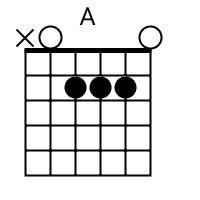
\includegraphics[width=3cm]{../Akordy/a.png}
%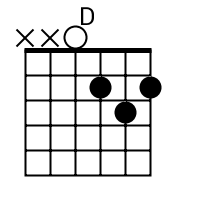
\includegraphics[width=3cm]{../Akordy/d.png}
%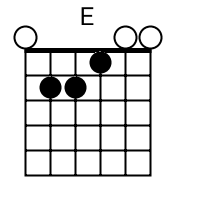
\includegraphics[width=3cm]{../Akordy/e.png}
%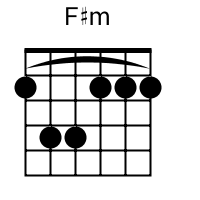
\includegraphics[width=3cm]{../Akordy/fxm.png}
%\end{figure}
